%% abtex2-modelo-trabalho-academico.tex, v-1.9.2 laurocesar
%% Copyright 2012-2014 by abnTeX2 group at http://abntex2.googlecode.com/ 
%%
%% This work may be distributed and/or modified under the
%% conditions of the LaTeX Project Public License, either version 1.3
%% of this license or (at your option) any later version.
%% The latest version of this license is in
%%   http://www.latex-project.org/lppl.txt
%% and version 1.3 or later is part of all distributions of LaTeX
%% version 2005/12/01 or later.
%%
%% This work has the LPPL maintenance status ``'maintained'.
%% 
%% The Current Maintainer of this work is the abnTeX2 team, led
%% by Lauro César Araujo. Further information are available on 
%% http://abntex2.googlecode.com/
%%
%% This work consists of the files abntex2-modelo-trabalho-academico.tex,
%% abntex2-modelo-include-comandos and abntex2-modelo-references.bib
%%

% ------------------------------------------------------------------------
% ------------------------------------------------------------------------
% abnTeX2: Modelo de Trabalho Academico (tese de doutorado, dissertacao de
% mestrado e trabalhos monograficos em geral) em conformidade com 
% ABNT NBR 14724:2011: Informacao e documentacao - Trabalhos academicos -
% Apresentacao
% ------------------------------------------------------------------------
% ------------------------------------------------------------------------

\documentclass[
	% -- opções da classe memoir --
	12pt,				% tamanho da fonte
	openright,			% capítulos começam em pág ímpar (insere página vazia caso preciso)
	twoside,			% para impressão em verso e anverso. Oposto a oneside
	a4paper,			% tamanho do papel. 
	% -- opções da classe abntex2 --
	%chapter=TITLE,		% títulos de capítulos convertidos em letras maiúsculas
	%section=TITLE,		% títulos de seções convertidos em letras maiúsculas
	%subsection=TITLE,	% títulos de subseções convertidos em letras maiúsculas
	%subsubsection=TITLE,% títulos de subsubseções convertidos em letras maiúsculas
	% -- opções do pacote babel --
	english,			% idioma adicional para hifenização
	% french,				% idioma adicional para hifenização
	% spanish,			% idioma adicional para hifenização
	brazil				% o último idioma é o principal do documento
	]{abntex2}

% ---
% Pacotes básicos 
% ---
\usepackage{lmodern}			% Usa a fonte Latin Modern			
\usepackage[T1]{fontenc}		% Selecao de codigos de fonte.
\usepackage[utf8]{inputenc}		% Codificacao do documento (conversão automática dos acentos)
\usepackage{lastpage}			% Usado pela Ficha catalográfica
\usepackage{indentfirst}		% Indenta o primeiro parágrafo de cada seção.
\usepackage{color}				% Controle das cores
\usepackage{graphicx}			% Inclusão de gráficos
\usepackage{microtype} 			% para melhorias de justificação
% ---
		
% ---
% Pacotes adicionais, usados apenas no âmbito do Modelo Canônico do abnteX2
% ---
\usepackage{lipsum}				% para geração de dummy text
% ---

% ---
% Pacotes de citações
% ---
\usepackage[brazilian,hyperpageref]{backref}	 % Paginas com as citações na bibl
\usepackage[alf]{abntex2cite}	% Citações padrão ABNT

% ---
% Pacotes adicionados por Rodrigo Cichetto
% ---
\usepackage{hyperref}
% CODES JS
\usepackage{listings}
\usepackage{color}
\definecolor{lightgray}{rgb}{.95,.95,.95}
\definecolor{darkgray}{rgb}{.4,.4,.4}
\definecolor{purple}{rgb}{0.65, 0.12, 0.82}

% ---
% CONFIGURAÇÃO RODRIGO
% ---
% CODES JS
\lstdefinelanguage{JavaScript}{
  keywords={typeof, new, true, false, catch, function, return, null, catch, switch, var, if, in, while, do, else, case, break},
  keywordstyle=\color{blue}\bfseries,
  ndkeywords={class, export, boolean, throw, implements, import, this},
  ndkeywordstyle=\color{darkgray}\bfseries,
  identifierstyle=\color{black},
  sensitive=false,
  comment=[l]{//},
  morecomment=[s]{/*}{*/},
  commentstyle=\color{purple}\ttfamily,
  stringstyle=\color{red}\ttfamily,
  morestring=[b]',
  morestring=[b]"
}

\lstset{
   language=JavaScript,
   backgroundcolor=\color{lightgray},
   extendedchars=true,
   basicstyle=\footnotesize\ttfamily,
   showstringspaces=false,
   showspaces=false,
   numbers=left,
   numberstyle=\footnotesize,
   numbersep=9pt,
   tabsize=4,
   breaklines=true,
   showtabs=false,
   captionpos=b
}


% --- 
% CONFIGURAÇÃO DE FIGURAS
% --- 
\graphicspath{ {imagens/} }

% --- 
% CONFIGURAÇÕES DE PACOTES
% --- 

% ---
% Configurações do pacote backref
% Usado sem a opção hyperpageref de backref
\renewcommand{\backrefpagesname}{Citado na(s) página(s):~}
% Texto padrão antes do número das páginas
\renewcommand{\backref}{}
% Define os textos da citação
\renewcommand*{\backrefalt}[4]{
	\ifcase #1 %
		Nenhuma citação no texto.%
	\or
		Citado na página #2.%
	\else
		Citado #1 vezes nas páginas #2.%
	\fi}%
% ---

% ---
% Informações de dados para CAPA e FOLHA DE ROSTO
% ---
\titulo{Desenvolvimento de aplicações com JavaScript}
\autor{Rodrigo Cichetto Monteiro}
\local{Brasil}
\data{2018, v-1.0.0}
\orientador{Leandro Carlos Fernandez}
\coorientador{Danielle Colturato}
\instituicao{%
  Universidade Paulista -- UNIP
  \par
  Faculdade de Ciência da Computação
  \par
  Programa de Graduação}
\tipotrabalho{Tese (Graduação)}
% O preambulo deve conter o tipo do trabalho, o objetivo, 
% o nome da instituição e a área de concentração 
\preambulo{Trabalho apresentado a UNIP - UNIVERSIDADE PAULISTA
como pré-requisito
para obtenção da Certificação de Conclusão do
Curso de Bacharelado em Ciência da Computação.
Orientador: Prof. \imprimirorientador}
% ---


% ---
% Configurações de aparência do PDF final

% alterando o aspecto da cor azul
\definecolor{blue}{RGB}{41,5,195}

% informações do PDF
\makeatletter
\hypersetup{
     	%pagebackref=true,
		pdftitle={\@title}, 
		pdfauthor={\@author},
    	pdfsubject={\imprimirpreambulo},
	    pdfcreator={LaTeX with abnTeX2},
		pdfkeywords={abnt}{latex}{abntex}{abntex2}{trabalho acadêmico}, 
		colorlinks=true,       		% false: boxed links; true: colored links
    	linkcolor=blue,          	% color of internal links
    	citecolor=blue,        		% color of links to bibliography
    	filecolor=magenta,      		% color of file links
		urlcolor=blue,
		bookmarksdepth=4
}
\makeatother
% --- 

% --- 
% Espaçamentos entre linhas e parágrafos 
% --- 

% O tamanho do parágrafo é dado por:
\setlength{\parindent}{1.3cm}

% Controle do espaçamento entre um parágrafo e outro:
\setlength{\parskip}{0.2cm}  % tente também \onelineskip

% ---
% compila o indice
% ---
\makeindex
% ---

% ----
% Início do documento
% ----
\begin{document}

% Retira espaço extra obsoleto entre as frases.
\frenchspacing 

% ----------------------------------------------------------
% ELEMENTOS PRÉ-TEXTUAIS
% ----------------------------------------------------------
% \pretextual

% ---
% Capa
% ---
\imprimircapa
% ---

% ---
% Folha de rosto
% (o * indica que haverá a ficha bibliográfica)
% ---
\imprimirfolhaderosto*
% ---

% ---
% Inserir a ficha bibliografica
% ---

% Isto é um exemplo de Ficha Catalográfica, ou ``Dados internacionais de
% catalogação-na-publicação''. Você pode utilizar este modelo como referência. 
% Porém, provavelmente a biblioteca da sua universidade lhe fornecerá um PDF
% com a ficha catalográfica definitiva após a defesa do trabalho. Quando estiver
% com o documento, salve-o como PDF no diretório do seu projeto e substitua todo
% o conteúdo de implementação deste arquivo pelo comando abaixo:
%
% \begin{fichacatalografica}
%     \includepdf{fig_ficha_catalografica.pdf}
% \end{fichacatalografica}
\begin{fichacatalografica}
	\vspace*{\fill}					% Posição vertical
	\hrule							% Linha horizontal
	\begin{center}					% Minipage Centralizado
	\begin{minipage}[c]{12.5cm}		% Largura
	
	\imprimirautor
	
	\hspace{0.5cm} \imprimirtitulo  / \imprimirautor. --
	\imprimirlocal, \imprimirdata-
	
	\hspace{0.5cm} \pageref{LastPage} p. : il. (algumas color.) ; 30 cm.\\
	
	\hspace{0.5cm} \imprimirorientadorRotulo~\imprimirorientador\\
	
	\hspace{0.5cm}
	\parbox[t]{\textwidth}{\imprimirtipotrabalho~--~\imprimirinstituicao,
	\imprimirdata.}\\
	
	\hspace{0.5cm}
		1. JavaScript.
		2. Desenvolvimento de aplicações.
		I. Orientador \imprimirorientador.
		II. Universidade Paulista -- UNIP.
		III. Faculdade de Ciência da Computação.
		IV. \imprimirtitulo 
		V. \imprimirautor
	
	\hspace{8.75cm} CDU 02:141:005.7\\
	
	\end{minipage}
	\end{center}
	\hrule
\end{fichacatalografica}
% ---

% ---
% Inserir errata
% ---
% \begin{errata}
% Elemento opcional da \citeonline[4.2.1.2]{NBR14724:2011}. Exemplo:

% \vspace{\onelineskip}

% FERRIGNO, C. R. A. \textbf{Tratamento de neoplasias ósseas apendiculares com
% reimplantação de enxerto ósseo autólogo autoclavado associado ao plasma
% rico em plaquetas}: estudo crítico na cirurgia de preservação de membro em
% cães. 2011. 128 f. Tese (Livre-Docência) - Faculdade de Medicina Veterinária e
% Zootecnia, Universidade de São Paulo, São Paulo, 2011.

% \begin{table}[htb]
% \center
% \footnotesize
% \begin{tabular}{|p{1.4cm}|p{1cm}|p{3cm}|p{3cm}|}
%   \hline
%    \textbf{Folha} & \textbf{Linha}  & \textbf{Onde se lê}  & \textbf{Leia-se}  \\
%     \hline
%     1 & 10 & auto-conclavo & autoconclavo\\
%    \hline
% \end{tabular}
% \end{table}
% \end{errata}
% ---

% ---
% Inserir folha de aprovação
% ---

% Isto é um exemplo de Folha de aprovação, elemento obrigatório da NBR
% 14724/2011 (seção 4.2.1.3). Você pode utilizar este modelo até a aprovação
% do trabalho. Após isso, substitua todo o conteúdo deste arquivo por uma
% imagem da página assinada pela banca com o comando abaixo:
%
% \includepdf{folhadeaprovacao_final.pdf}
%
\begin{folhadeaprovacao}

  \begin{center}
    {\ABNTEXchapterfont\large\imprimirautor}

    \vspace*{\fill}\vspace*{\fill}
    \begin{center}
      \ABNTEXchapterfont\bfseries\Large\imprimirtitulo
    \end{center}
    \vspace*{\fill}
    
    \hspace{.45\textwidth}
    \begin{minipage}{.5\textwidth}
        \imprimirpreambulo
    \end{minipage}%
    \vspace*{\fill}
   \end{center}
        
   Trabalho aprovado. \imprimirlocal, 24 de novembro de 2018:

   \assinatura{\textbf{\imprimirorientador} \\ Orientador} 
   \assinatura{\textbf{Professor} \\ Convidado 1}
   \assinatura{\textbf{Professor} \\ Convidado 2}
   %\assinatura{\textbf{Professor} \\ Convidado 3}
   %\assinatura{\textbf{Professor} \\ Convidado 4}
      
   \begin{center}
    \vspace*{0.5cm}
    {\large\imprimirlocal}
    \par
    {\large\imprimirdata}
    \vspace*{1cm}
  \end{center}
  
\end{folhadeaprovacao}
% ---

% ---
% Dedicatória
% ---
% \begin{dedicatoria}
%    \vspace*{\fill}
%    \centering
%    \noindent
%    \textit{ Este trabalho é dedicado às crianças adultas que,\\
%    quando pequenas, sonharam em se tornar cientistas.} \vspace*{\fill}
% \end{dedicatoria}
% ---

% ---
% Agradecimentos
% ---
% \begin{agradecimentos}
% Os agradecimentos principais são direcionados à Gerald Weber, Miguel Frasson,
% Leslie H. Watter, Bruno Parente Lima, Flávio de Vasconcellos Corrêa, Otavio Real
% Salvador, Renato Machnievscz\footnote{Os nomes dos integrantes do primeiro
% projeto abn\TeX\ foram extraídos de
% \url{http://codigolivre.org.br/projects/abntex/}} e todos aqueles que
% contribuíram para que a produção de trabalhos acadêmicos conforme
% as normas ABNT com \LaTeX\ fosse possível.

% Agradecimentos especiais são direcionados ao Centro de Pesquisa em Arquitetura
% da Informação\footnote{\url{http://www.cpai.unb.br/}} da Universidade de
% Brasília (CPAI), ao grupo de usuários
% \emph{latex-br}\footnote{\url{http://groups.google.com/group/latex-br}} e aos
% novos voluntários do grupo
% \emph{\abnTeX}\footnote{\url{http://groups.google.com/group/abntex2} e
% \url{http://abntex2.googlecode.com/}}~que contribuíram e que ainda
% contribuirão para a evolução do \abnTeX.
% \end{agradecimentos}
% ---

% ---
% Epígrafe
% ---
\begin{epigrafe}
    \vspace*{\fill}
	\begin{flushright}
		\textit{``Cada sonho que você deixa pra trás,\\
		é um pedaço do seu futuro que deixa de existir. \\
		(Steve Jobs)}
	\end{flushright}
\end{epigrafe}
% ---

% ---
% RESUMOS
% ---

% resumo em português
\setlength{\absparsep}{18pt} % ajusta o espaçamento dos parágrafos do resumo
\begin{resumo}
%  Segundo a \citeonline[3.1-3.2]{NBR6028:2003}
Fazendo parte das três principais tecnologias que movem a internet, sendo elas HTML, CSS e claro o JavaScript, não é mais uma linguagem voltada somente para desenvolvedores front-end, mas sim uma obrigação para todo desenvolvedor, que tem como obrigação conhecer pelo menos o básico de JS. Nos últimos tempos a linguagem ganhou muita importância em quaisquer cenários, e vem sendo utilizada em sites, aplicações, mobile, servidores, automação de testes, automação de tarefas, internet das coisas, entre outros. Este trabalho tem como principal objetivo atualizar o leitor através de um compilado de informações sobre as tendências do que mais vem sendo utilizado para a construção de aplicações utilizando a linguagem, mostrando os frameworks mais recentes e mais famosos. Mas lembre-se com grandes poderes vem grandes responsabilidades.

 \vspace{\onelineskip}

 \textbf{Palavras-chaves}: javascript, typescript, frameworks
\end{resumo}

% resumo em inglês
\begin{resumo}[Abstract]
 \begin{otherlanguage*}{english}

Being part of the three main technologies that move the internet, being HTML, CSS and clear JavaScript, is no longer a language aimed only at front-end developers, but rather an obligation for every developer, who has to know at least the basics of JS. In recent times the JavaScript language has gained a lot of importance in any scenarios involving programming, and has been used in websites, applications, servers, automation of tests, automation of tasks, internet of things, among others. This work has as main objective to update the reader through a compilation of information about the trends of what is being used to build applications using the language, showing the latest and most famous frameworks. But remember with great powers comes great responsibilities.

   \vspace{\onelineskip}
 
   \noindent 
   \textbf{Key-words}: javascript, typescript, frameworks
 \end{otherlanguage*}
\end{resumo}
% ---
% inserir lista de ilustrações
% ---
\pdfbookmark[0]{\listfigurename}{lof}
\listoffigures*
\cleardoublepage
% ---

% ---
% inserir lista de tabelas
% ---
% \pdfbookmark[0]{\listtablename}{lot}
% \listoftables*
% \cleardoublepage
% ---

% ---
% inserir lista de abreviaturas e siglas
% ---
\begin{siglas}
%   \item[ABNT] Associação Brasileira de Normas Técnicas
%   \item[abnTeX] ABsurdas Normas para TeX
  \item[JS] JavaScript
  \item[HTML] Abreviação para \textit{HyperText Markup Language}, que em português significa Linguagem de Marcação de Hipertexto.
  \item[DOM] Abreviação para \textit{Document Object Model}, que em português significa Modelo de Objetos e Documentos.
  \item[CSS] Abreviação para \textit{Cascading Style Sheets}, que em português significa Folhas de Estilo em Cascata.
  \item[ECMA] Abreviação para \textit{European Computer Manufacturers Association}, que em português significa Associação Européia de Fabricantes de Computadores.
  \item[API] Abreviação para \textit{Application Programming Interface}, que em português significa Interface de programação de aplicações.
\end{siglas}
% ---

% ---
% inserir lista de símbolos
% ---
% \begin{simbolos}
% 	\item
% %   \item[$ \in $] Pertence
% \end{simbolos}
% ---

% ---
% inserir o sumariopr
% ---
\pdfbookmark[0]{\contentsname}{toc}
\tableofcontents*
\cleardoublepage
% ---

% TODO inserir SOBRE O AUTOR

% ----------------------------------------------------------
% ELEMENTOS TEXTUAIS
% ----------------------------------------------------------
\textual

% ----------------------------------------------------------
% Introdução (exemplo de capítulo sem numeração, mas presente no Sumário)
% ----------------------------------------------------------
% \chapter*[Introdução]{Introdução}
% \addcontentsline{toc}{chapter}{Introdução}
\chapter{Introdução}
% ----------------------------------------------------------

Inicialmente implementada com o objetivo no desenvolvimento web para o lado do
cliente, a linguagem criada por Brendan Eich enquanto trabalhou na Netscape se tornou
uma das linguagens mais populares da atualidade, sendo a terceira camada do bolo quando
se fala de tecnologias web, das quais HTML e CSS também fazem parte. 

Com navegadores cada vez mais modernos a tendência é que nossos sites também fiquem cada vez mais sofisticados.

Todo projeto que iniciamos existe uma origem, uma necessidade e um 
problema a ser resolvido. Há algum tempo, um grande problema ganhou 
atenção: a reutilização de trechos de código. São módulos de código 
(trechos em HTML, CSS, JavaScript, etc) que juntos criam padronizações 
e organizações, mas sobretudo flexibilidade. São os chamados frameworks.

Nos últimos anos a linguagem JavaScript ganhou maior importância, com o
surgimento de bibliotecas e frameworks que possibilitaram o desenvolvimento de não
somente web sites mas também aplicativos, single page applications, programas desktop,
progressive web apps e muito mais. Sendo alguns deles Angular, React, Vue, jQuery e
Node.js.

Talvez nenhuma outra linguagem tenha conseguido ganhar tanta atenção dos desenvolvedores como o JavaScript. Em busca de  sua identidade a linguagem foi a única que conseguiu se enraizar nos navegadores, e atualmente também passou a se empoderar dos servidores de alta performance através do Node.js.

O surgimento do Node.js possibilitou um novo mundo para os desenvolvedores,
levando a linguagem para um novo patamar. Criado com um modelo não bloqueante na
entrada e saída de dados, possibilitou que a linguagem fosse levada agora também para
aplicações back-end, ou seja, para o server-side (lado do servidor).

Com o tempo a Microsoft desenvolveu o TypeScript, que de uma forma simples é o
JavaScript acrescido de tipagem de dados, ou seja, agora erros podem ser detectados
durante a digitação do código, sem dúvidas podemos considerar o TypeScript como uma
evolução do JavaScript.

Este trabalho tem como objetivo atualizar o leitor do que há de mais novo no desenvolvimento com a linguagem JavaScript, para melhor compreensão do conteúdo apresentado é necessário conhecimento prévio básico da linguagem. 


% ----------------------------------------------------------
% PARTE 1. JAVASCRIPT
% ----------------------------------------------------------
\part{A linguagem JavaScript}
% ----------------------------------------------------------
% ---
% Capitulo O Básico sobre JS
% ---
\chapter{O Básico sobre JS}

JavaScript é uma linguagem de programação dinâmica interpretada, inicialmente utilizada pelos navegadores para execução de \textit{scripts} no lado do cliente, ou seja, no seu \textit{browser}. Os \textit{scripts} são incorporados a páginas HTML tendo como função adicionar interatividade para o usuário.

Atualmente, é praticamente impossível imaginar a internet sem a existência do JavaScript, certamente você já se deparou com alguns dos exemplos como os famosos carrosseis (Figura \ref{fig:JSExampleCarrousel}, página \pageref{fig:JSExampleCarrousel}), as tão importantes validações de formulários (Figura \ref{fig:JSExampleValidation}, página \pageref{fig:JSExampleValidation}), ou até mesmo o \textit{modal} (Figura \ref{fig:JSExampleModal}, página \pageref{fig:JSExampleModal}) que mostram a aplicação da linguagem em \textit{web sites}.

A web está infestada de códigos JavaScript, pode ter certeza de que diariamente muitos \textit{scripts} estão sendo executados durante uma pesquisa no Google, seu tempo no Facebook, acesso a seu banco na internet, ou até mesmo para leitura de uma notícia em um portal. Seu uso primário na web é de funções incluídas no HTML que interagem com o Modelo de Objetos e Documentos (DOM) da página.

DOM é uma interface de programação utilizada para documentos HTML, ele fornece a representação e interação com objetos os estruturando em nós de uma árvore chamada de Árvore DOM. É assim que o JavaScript consegue manusear as estruturas, estilos e conteúdos dos elementos presentes no HTML. Vale ressaltar que ele não faz parte da linguagem JavaScript, pois também pode ser acessado por outras linguagens.

O JavaScript apresenta uma sintaxe simples que facilita o aprendizado, mas não confunda pois a primeira vista muitos desenvolvedores podem acreditar que a linguagem é defeituosa ou esquisita, pois não compreendem o real poder que se esconde por trás desta simplicidade. 

% \section{Caracteristicas}
Inicialmente classificada como linguagem do tipo \textit{client side}, é por si só uma linguagem compacta, mas muito flexível, com comportamentos diferenciados das demais ela permite, por exemplo, que um objeto tenha seus atributos adicionados ou removidos em tempo de execução, o que não é muito comum para desenvolvedores de outras linguagens.

É uma linguagem interpretada, pois seus comandos são executados sem que haja necessidade de compilação, tendo como interpretador de \textit{script} o \textit{browser} do usuário. Sendo assim independente de plataformas, como os comandos são interpretados pelo navegador do usuário é irrelevante se o usuário está utilizando Windows, Linux ou Mac OS.

Sua tipagem é dinâmica, ou seja, tipos são associados com valores. Por exemplo, uma variável pode ser associada a um número e posteriormente associada a um texto.

Baseada em objetos, no JavaScript os objetos são matrizes associativas, ou seja \verb|obj.a = 10| e \verb|obj["a"] = 10| são equivalentes, sendo a única diferença a própria sintaxe.

As funções em JS são tratadas como objetos, possuindo métodos e propriedades, podendo assim serem atríbuidas a variáveis, retornadas como objetos, ou até mesmo passadas como argumentos para outras funções, o que é chamado de aninhamento de funções.

Com JavaScript também é possível a detecção de eventos, sempre que algo de importante acontece é disparado um evento, o clique de um botão, o preenchimento de um campo de formulário, a movimentação do mouse, são alguns exemplos dos eventos que são disparados. Isso nos permite reagir a estes eventos deixando assim que nossa aplicação deixe de ser estática.

A linguagem possui grande tolerância a erros, uma vez que conversões automáticas são realizadas durante suas operações.

Podemos executar códigos JS de várias formas na web, sendo uma delas pelo próprio console do navegador pressionando as teclas F12, importando um script em uma página HTML, ou até mesmo envolvendo o trecho de código na tag <script>.

No início da internet as páginas não eram nada interativas, documentos apresentavam seu conteúdo exatamente como foram criados para serem exibidos no navegador e só. O JavaScript revolucionou o que podemos fazer, hoje não só na web, mas praticamente em todas as áreas que se possa programar. 

No próximo capítulo abordaremos de como surgiu a linguagem, como ela evoluiu e atua no presente e a necessidade de padronizações.

\begin{figure}[h]
	\centering

	\caption{\textit{Carrousel} - Um componente de apresentação de slides para percorrer imagens ou slides de texto - como um carrossel. -- Exemplo de aplicação do JS} \label{fig:JSExampleCarrousel}
    
\includegraphics[scale=0.4]{js-example-carrousel} \\
    Fonte: {Bootstrap \url{https://getbootstrap.com/docs/4.1/components/carousel/}}

    \caption{\textit{Validation} - Validação de formulários -- Exemplo de aplicação do JS} \label{fig:JSExampleValidation}
    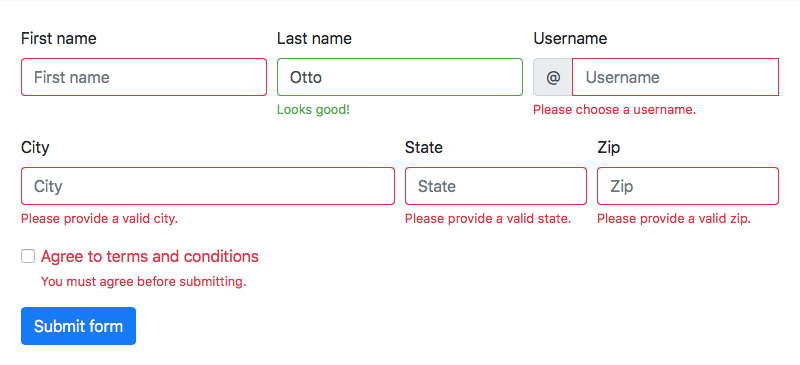
\includegraphics[scale=0.45]{js-example-validation} \\
    Fonte: {Bootstrap \url{https://getbootstrap.com/docs/4.1/components/forms/}}
	
    \caption{\textit{Modal} - Caixas de diálogo para notificações ao usuário. -- Exemplo de aplicação do JS} \label{fig:JSExampleModal}
    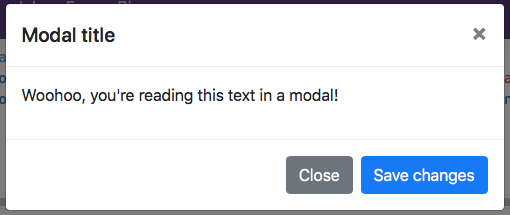
\includegraphics[scale=0.5]{js-example-modal} \\
    Fonte: {Bootstrap \url{https://getbootstrap.com/docs/4.1/components/modal/}}

\end{figure}

% ---
% Capitulo JavaScript não é Java
% ---
\chapter{JavaScript não é Java}
Acredite JavaScript não é Java, criada em 1995 por Brendan Eich a linguagem ganhou esse nome somente por estratégia publicitária, na época a recém lançada linguagem Java tinha muita sucesso. O que causou muitas confusões que existem até hoje para aqueles que iniciam no mundo da programação, pois esses indivíduos pensam que as linguagens são iguais ou que o JavaScript é uma versão mais simples do Java, o que não é verdade. É muito importante deixar claro que Java e JavaScript são linguagens diferentes e com propósitos também distintos, a única coisa parecida entre elas é o nome.

Brendan Eich, trabalhava na Netscape quando desenvolveu em apenas 10 dias uma linguagem de programação simples com o intuito de atrair novos programadores para ela.

\begin{figure}[h]
    \centering
    \label{fig:BrendanEich}
    \caption{\textit{Brendan Eich} - Criador do JavaScript.}
    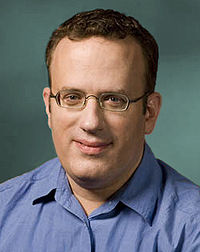
\includegraphics[scale=0.6]{brendan-eich} \\
    Fonte: {Wikipedia \url{https://pt.wikipedia.org/wiki/}}
	% https://pt.wikipedia.org/wiki/Brendan_Eich
\end{figure}

Originalmente desenvolvida com o nome Mocha (nome de um tipo de café), posteriormente teve seu nome modificado para LiveScript e, por fim, JavaScript em 4 de dezembro de 1995, nome pelo qual ficou tão conhecida.

O JavaScript teve grande influencia da linguagem C, suportando elementos de sintaxe de programação estruturada do C (por exemplo while, if, switch) ambas diferem expressões e comandos, temos como exceção o escopo em blocos, que em seu lugar o JS utiliza escopos a níveis de funções. Uma diferença curiosa do C é que a quebra de linha termina automaticamente o comando, sendo assim o ponto e vírgula opcional ao fim do comando.

Logo a linguagem adquiriu ampla aceitação e cresceu cada vez mais, desde então o JavaScript se tornou a linguagem de programação mais popular da web. Suportada por todos os navegadores, a linguagem é responsável por praticamente qualquer tipo de dinamismo que queiramos em nossas páginas.

% ---
% Capitulo A linguagem nos dias atuais
% ---
\chapter{A linguagem nos dias atuais}

Se existe alguma linguagem que evoluiu nos últimos tempos, essa linguagem é o JavaScript. Conforme a linguagem evoluiu se tornou mais poderosa e independente do navegador. Isso possibilitou que a linguagem fosse utilizada não somente para a web como \textit{client side} mas agora em vários lugares. 

\section{JavaScript além dos navegadores}

Inicialmente tratada como um extra para os navegadores, podemos dizer que a linguagem caminhou com o avanço da tecnologia, isso possibilitou o uso da linguagem em diversas áreas sendo elas:

\begin{enumerate}[label=\alph*)]
\item Aplicações web
\item Aplicativos mobile 
\item Automação de testes e de tarefas
\item Controle de hardware
\item Desenvolvimento de jogos
\item Internet das coisas
\item Realidade virtual e aumentada
\item Softwares desktop
\item Servidores 
\end{enumerate}

Praticamente tudo que envolve programação o JavaScript está presente, para criar um software desktop existe por exemplo o \textit{framework} Electron (https://electronjs.org), desenvolvido pelo GitHub ele possibilita criar aplicativos desktop multiplataforma através do JavaScript. No desenvolvimento de jogos a \textit{engine} Unity (https://unity3d.com/pt) é uma das plataformas que oferecem suporte a linguagem.

Hoje grandes empresas como Google, Microsoft, Netflix, Uber e Linkedin usam JavaScript até mesmo no \textit{back-end}. 

Isso acabou impactando o mundo dos desenvolvedores, fazendo com que seja obrigatório todo programador saber pelo menos o básico da linguagem, mesmo atuando na área de \textit{back-end} ou até mesmo de teste.

\section{ECMA}
% TODO: INSERIR PARAGRAFO EXPLICANDO COMO FUNCIONA PARA ENVIAR PROPOSTA PARA ECMA https://tableless.com.br/entendendo-o-async-e-o-await-em-javascript/
Atualmente a linguagem se encontra na 9ª edição chamada de ECMAScript 2018, finalizada em Junho de 2018, suas últimas contribuições de maior expressão foram a inclusão dos operadores \textit{await} e \textit{async}, possibilitando agora que a linguagem trabalhe com funções assíncronas de uma maneira simples. 
% TODO CONTINUAR COM NOVAS FUNCIONALIDADES DA LINGUAGEM
% TODO APONTAR NOVOS RUMOS DA LINGUAGEM, SUPORTE MOBILE... (https://www.youtube.com/watch?v=851mizGnr_Y)

Pela linguagem rodar em ambientes que podem variar, algo importante a considerar é a compatibilidade entre os navegadores. Para isso é necessário um padrão a seguir, tal criado e mantido até hoje pelo ECMA Internacional.

Já em 1996 a Netscape, detentora do JavaScript, anúnciou que submetia a linguagem para o ECMA Internacional como candidata a padrão industrial, resultando então no ECMAScript.

Padronização que define a estrutura da linguagem, seus comportamentos e comandos, dando assim um padrão aos interpretadores da linguagem. 

Com participação colaborativa de empresas que implementam o \textit{run-time} da linguagem, como Mozilla, Google, Microsoft e Apple, além da participação de desenvolvedores da comunidade, o ECMA coordena e faz o trabalho de desenvolvimento contínuo e descentralizado do JS.

Em seu site \url{http://www.ecma-international.org/publications/standards/Ecma-262.htm}, a ECMA disponibiliza informações como versão atual e a documentação da linguagem, porém aconselho a buscar documentações na internet, uma boa referência a seguir é o site da Mozilla \url{https://developer.mozilla.org/pt-BR/docs/Web/JavaScript}, ou também o site da W3Schools \url{https://www.w3schools.com/jsref/default.asp}. 

A 10ª edição já está em desenvolvimento, devendo chegar até o final de Junho no ano de 2019, sendo chamada de ECMAScript 2019.

\section{Futuro da linguagem}


% ----------------------------------------------------------
% PARTE 2. TYPESCRIPT
% ----------------------------------------------------------
\part{O TypeScript}
% ----------------------------------------------------------
% ---
% Capitulo O JS com poderes
% ---
\chapter{O JS com poderes}

O TypeScript é um \textit{superset} para o JavaScript criado pela Microsoft, que  permite ao desenvolvedor aplicar conceitos de orientação a objetos a linguagem, ou seja, é o próprio JS com algumas funcionalidades a mais. Assim, podemos afirmar que todo código JavaScript é um TypeScript válido, uma vez que o código em TypeScript, é convertido no final para código JavaScript através de um processo de transpilação.


% ----------------------------------------------------------
% PARTE 3. Criando aplicações modernas
% ----------------------------------------------------------
\part{Criando aplicações modernas}
% ----------------------------------------------------------
% TODO ADICIONAR PROGRAMAÇÃO REATIVA...
% ---
% Capitulo Web Services
% ---
\chapter{Web Services}

% ---
% Capitulo Compiladores
% ---
% \chapter{Compiladores}

% \lipsum[1]

% \lipsum[2-3]

% ----------------------------------------------------------
% PARTE 4. Frameworks, bibliotecas e tecnologias
% ----------------------------------------------------------
\part{Frameworks, bibliotecas e tecnologias}
% ----------------------------------------------------------
% ---
% Capitulo A pilha
% ---
\chapter{Frameworks são hypes}

% TODO Conceito em si de o que é um framework
Um framework, é um conjunto de bibliotecas que tem o objetivo de facilitar o desenvolvimento ditando o fluxo da aplicação. De forma mais simples pode ser visto como o esqueleto da aplicação.

O principal benefício no uso de \textit{frameworks} em empresas é a capacidade de economizar tempo, mas também inclui a facilidade de aprendizado, por normalmente obter documentações e comunidades, padronização de código, contribuindo assim para que o código seja mais legível tornando a manutenção mais facil, além de outras muitas vantagens.

JavaScript é bem famoso na comunidade por ter muitos \textit{frameworks}, com certeza você já ouviu falar de React, Vue, Angular
% TODO continuar...

Mas nem tudo são flores, quando você escolhe usar um \textit{framework} para a criação do seu projeto acaba causando depêndencia de bibliotecas, tornando mais complicado em casos de migração além de códigos desnecessários, que podem deixar seu sistema mais pesado.

% TODO Passar a ideia de que o objetivo é entender como o framework funciona pois ele apenas é um conjunto de código js que alguém desenvolveu e que foi criado para facilitar o desenvolvimento (para não reiventarmos a roda).
Muitas empresas exigem o conhecimento de \textit{frameworks} para que o funcionário se adeque ao desenvolvimento da equipe, mas uma dica é não foque somente em aprender os comandos de um \textit{framework}, pois os mesmos são \textit{hypes}, quando digo isso significa que com o tempo novos serão criados e todos irão migrar para o que há de mais novo. Tenha como objetivo entender como ele funciona, suas engrenagens e conceitos, pois nada mais é do que um conjunto de código criado por alguém visando facilitar nosso desenvolvimento, para não termos que reiventarmos a roda.

Entenda, não estou dizendo que eles não são importantes, mas sim que se você sabe a linguagem em si, e como utilizá-la se dará bem com qualquer \textit{framework}, o que é o mais importante.

Invista seu tempo em aprender a linguagem, não se apegue muito a frameworks. 
% ---
% Capitulo A pilha
% ---
\chapter{A pilha MEAN}

Das iniciais das ferramentas MongoDB, Express, Angular e Node.js, MEAN é o nome dado quando integramos todas essas ferramentas para desenvolver uma aplicação. Sendo que todas utilizam como linguagem o JavaScript, possibilitando que um programador da linguagem tenha maior facilidade para trabalhar em todas as partes da aplicação, seja front-end, back-end ou banco de dados.

\begin{figure}[h]
	\centering

	\caption{\textit{MEAN Stack} - Fluxo das ferramentas que integram o MEAN} \label{fig:MEANStackFlow}
    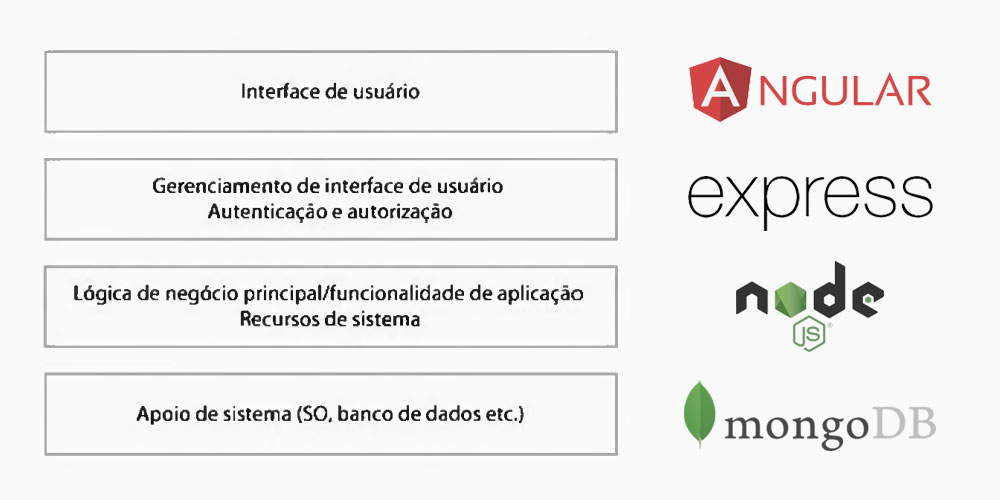
\includegraphics[scale=0.5]{mean-stack-flow} \\
    Fonte: {orangemantra \url{https://www.orangemantra.com/blog/utilize-the-simplicity-of-mean-stack-technology-for-your-next-project/}}
	% https://www.orangemantra.com/blog/wp-content/uploads/2016/06/mean-stack.jpg

\end{figure}

\section{MongoDB}

Um banco de dados flexível, poderoso, escalonável e de alta performance orientado a documentos. Lançado em 2009, escrito em C++, o MongoDB é gratuito e de código aberto.

Por ser orientado à documentos JSON, ou seja, retém os dados usando pares de chave/valor, podemos modelar dados de forma mais natural, utilizando a forma como os dados realmente serão utilizados em nossa aplicação, ao invés de criar várias ligações entre tabelas, o que o dá a característica ao MongoDB de banco não-relacional.

Para a execução de comandos no Mongo, existe um console que executa códigos JavaScript. Por esse motivo, desenvolvedores da linguagem terão facilidade em manter um banco MongoDB.

Em uma aplicação desenvolvida em cima do MEAN Stack o Mongo tem a responsabilidade de persistir os dados.

\subsection{Instalação}

Para instalar o MongoDB, basta acessar o link \url{https://www.mongodb.com/download-center} e baixar o instalador de acordo com seu sistema operacional.

É necessário criar um diretório para o Mongo escrever seus arquivos, crie a pasta "data" e dentro dela a pasta "db", se você utiliza Linux ou Mac pode utilizar os seguintes comandos:

\begin{itemize}
% mkdir -p /data/db
% chown -R $USER:$USER /data/db     ou     chown -R \textdollar USER:\textdollar USER /data/db
\item \verb|mkdir -p /data/db|
\item \verb|chown -R $USER:$USER /data/db|
\end{itemize}

Para iniciar o servidor Mongo, acesse o diretório de instalação pelo terminal e execute o comando bin/mongod.exe se utilizar Windows ou bin/mongod se utilizar Linux ou Mac. Logo após é possível iniciar o MongoDB pelo comando bin/mongo , caso esteja em um ambiente Windows execute bin/mongo.exe .

Através deste terminal podemos criar bancos de dados, documentos e coleções. Se em qualquer momento for preciso obter ajuda, basta dar o comando \verb|help| na linha de comando do terminal do Mongo.

\subsection{Primeiros passos}

Por padrão o terminal do Mongo inicia conectado ao banco de dados \verb|test|. Para mudarmos para outro banco de dados utilizamos o comando \verb|use nome_do_banco|. Caso o banco indicado não exista, o Mongo criará um novo assim que dados forem incluídos nele.

\textit{Insert}, através da função \verb|insert()| insere novos dados e pode receber como parâmetro um objeto JSON ou um array de objetos.

\begin{lstlisting}[language=javascript]
// Exemplo insert
db.nome_do_banco.insert()
\end{lstlisting}

\textit{Find}, através da função \verb|find()|, busca por objetos inseridos em uma \textit{collection}, podendo receber como parâmetro um objeto com os critérios de filtragem, ou nenhum para retornar todos os objetos.
 
\begin{lstlisting}[language=javascript]
// Exemplo find
db.nome_do_banco.find()
\end{lstlisting}

\textit{Update}, através da função \verb|update()| atualiza os dados, recebendo dois parâmetros, sendo o primeiro a condição para achar o documento, e o segundo o novo documento.

\begin{lstlisting}[language=javascript]
// Exemplo update
db.nome_do_banco.update()
\end{lstlisting}

\textit{Remove}, através da função \verb|remove()| remove os dados, podendo passar um parâmetro para informar qual objeto remover ou nenhum para remover todos, caso esse seja seu objetivo, também é possível utilizar o comando \verb|drop()|.

\begin{lstlisting}[language=javascript]
// Exemplo remove
db.nome_do_banco.remove()
// Exemplo drop
db.nome_do_banco.drop()
\end{lstlisting}


\section{Express}

Express é um \textit{framework} web rápido, flexível e minimalista para Node.js inspirado no Sinatra, um \textit{framework} para Ruby. Ele facilita o desenvolvimento de aplicações web e APIs, tanto pequenas quanto mais robustas, tornando fácil escalonar aplicações criadas com ele.

Com um conjunto de métodos utilitários HTTP e middlewares a seu dispor, criar uma API robusta utilizando Express é rápido e fácil.

\subsection {Primeiros passos}

Para criarmos um servidor com o Express, necessitamos primeiro do Node.js e o NPM instalados (veja como instalalos no capítulo ...) e então criar um arquivo com as seguintes linhas de código.

No terminal execute o comando \verb|npm install express| dentro do diretório do seu projeto. Desta maneira conseguimos importar o express para nosso código. E então é só criar um arquivo \verb|app.js| com o código abaixo.

\begin{lstlisting}[language=javascript]
import express from 'express';

let app = express();
const PORT = 3000;

app.get('/', (req, res) => {
   res.send('Hello World');
});

app.listen(PORT);
console.log(`Servidor disponivel na porta ${PORT}`);
\end{lstlisting}

\subsection{Express Generator}

Com apenas o comando \verb|express nome_da_app| do Express Generator ele já estrutura uma aplicação Express simples. Após a execução do comando ele irá criar um novo diretório com o nome da aplicação informado anteriormente, contendo arquivos e dependências necessárias. 

Antes de iniciarmos o servidor Express devemos instalar as dependências através do comando \verb|npm install| que irá baixar as dependências de acordo com o arquivo \verb|package.lock| gerado anteriormente. Enfim é hora de iniciar a aplicação executando o comando \verb|npm start| e acessá-la pelo endereço \href{http://localhost:3000}{http://localhost:3000}.

\begin{figure}[h]
	\centering

	\caption{Aplicação gerada pelo Express Generator} \label{fig:ExpressGeneratorApp}
    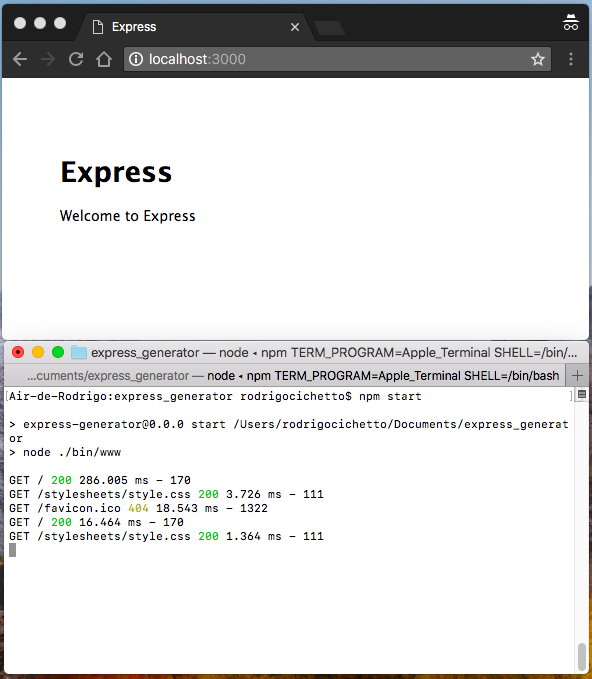
\includegraphics[scale=0.5]{express-generator-app} \\

\end{figure}

Essa página só é exibida porque no arquivo \verb|routes/index.js| está configurado a rota padrão para que renderize o arquivo \verb|views/index.jade| passando o título com o valor Express, sendo interpretado pela \textit{template engine} JADE, configurada por padrão pelo Express Generator.

Para saber mais opções de geração de estruturas através do Express Generator, execute o comando \verb|express -h|.

\section{Angular}

Angular é um framework JavaScript de código aberto, mantido pela Google. E tem como princípio "\textit{One framework. Mobile and desktop}", que basicamente significa utilizarmos o Angular para criar nossa aplicação web e também aplicações para dispositivos móveis.

O \textit{framework} utiliza TypeScript como linguagem, isso pode nos ajudar a manter melhor um projeto grande, já que a tipagem de variáveis nos força a sempre utilizar uma váriavel ou objeto do mesmo tipo, dando assim de certa forma uma garantia de que não teremos problemas ao acessar algum dado.

\subsection{Angular CLI} 


\section{Node.js}

O Node.js é uma plataforma de desenvolvimento construída sobre a linguagem JavaScript, por sua natureza assíncrona, exectuada pelo interpretador V8 criado pela Google e utilizado no Google Chrome, focado em migrar a linguagem para servidores. Foi criado pensando em um modelo não bloqueante para as operações de entrada e saída de dados (I/O - \textit{Input and Output}).

Neste modelo, as operações de I/O não bloqueiam o atendimento aos outros clientes, ou seja, quando são feitas operações como uma leitura no disco ou consulta de banco de dados, as requisições de outros clientes vão sendo enfileiradas. Após o processamento ser finalizado e respondido ao primeiro cliente, o próximo cliente é atendido.

\subsection{NPM}

O \textit{Node Package Manager}, mais conhecido como npm é o gerenciador de pacotes do Node.js. Com ele podemos fazer download de códigos, bibliotecas e \textit{frameworks} que nossos projetos podem usar, ou até mesmo ferramentas que exerçam alguma função em nosso sistema operacional.

O arquivo \verb|package.json| é responsável por gerenciar os pacotes cujo nosso projeto depende. Ele basicamente serve como uma lista para as dependências que nosso projeto necessita. Executando o comando \verb|npm install| automaticamente todas as dependências listadas serão baixadas.

Isso também nos ajuda a padronizar as versões de nossas dependências, facilitando informar os requisitos mínimos e atualizações, garantindo assim que todos os desenvolvedores terão a mesma versão em suas máquinas. Outra vantagem é para que outro desenvolvedor tenha acesso a nosso código, basta enviar o código em si, sem se preocupar com as dependências, pois basta ele executar o comando \verb|npm install| para fazer o download. 


% ----------------------------------------------------------
% PARTE 5. Conclusão
% ----------------------------------------------------------
\part{Conclusão}
% ----------------------------------------------------------

% ----------------------------------------------------------
% Finaliza a parte no bookmark do PDF
% para que se inicie o bookmark na raiz
% e adiciona espaço de parte no Sumário
% ----------------------------------------------------------
%\phantompart

% ---
% Considerações finais (outro exemplo de capítulo sem numeração e presente no sumário)
% ---
\chapter*[Considerações finais]{Considerações finais}
\addcontentsline{toc}{chapter}{Considerações finais}
% ---

\lipsum[31-33]

% ----------------------------------------------------------
% ELEMENTOS PÓS-TEXTUAIS
% ----------------------------------------------------------
\postextual
% ----------------------------------------------------------

% ----------------------------------------------------------
% Referências bibliográficas
% ----------------------------------------------------------
\bibliography{abntex2-modelo-references}

% ----------------------------------------------------------
% Glossário
% ----------------------------------------------------------
%
% Consulte o manual da classe abntex2 para orientações sobre o glossário.
%
%\glossary

% ----------------------------------------------------------
% Apêndices
% ----------------------------------------------------------

% ---
% Inicia os apêndices
% ---
% \begin{apendicesenv}

% % Imprime uma página indicando o início dos apêndices
% \partapendices

% % ----------------------------------------------------------
% \chapter{Quisque libero justo}
% % ----------------------------------------------------------

% \lipsum[50]

% % ----------------------------------------------------------
% \chapter{Nullam elementum urna vel imperdiet sodales elit ipsum pharetra ligula
% ac pretium ante justo a nulla curabitur tristique arcu eu metus}
% % ----------------------------------------------------------
% \lipsum[55-57]

% \end{apendicesenv}
% ---


% ----------------------------------------------------------
% Anexos
% ----------------------------------------------------------

% ---
% Inicia os anexos
% ---
% \begin{anexosenv}

% % Imprime uma página indicando o início dos anexos
% \partanexos

% % ---
% \chapter{Morbi ultrices rutrum lorem.}
% % ---
% \lipsum[30]

% % ---
% \chapter{Cras non urna sed feugiat cum sociis natoque penatibus et magnis dis
% parturient montes nascetur ridiculus mus}
% % ---

% \lipsum[31]

% % ---
% \chapter{Fusce facilisis lacinia dui}
% % ---

% \lipsum[32]

% \end{anexosenv}

%---------------------------------------------------------------------
% INDICE REMISSIVO
%---------------------------------------------------------------------
%\phantompart
\printindex
%---------------------------------------------------------------------

\end{document}